\experiment{8}{%
    Calculate the correlation coefficient for two variable using an appropriate method. Interpret the strength and direction of the relationship.
}

\subsection{Calculating correlation coefficient}

We'll be using Karl Pearson correlation of calculation the coefficients, because our data is fairly linear(observed in exp. 7) and has no outliers(observed in exp. 4, 5, \& 6).

\subsubsection*{i) Marks vs StudyHours}

\begin{lstlisting}[style=python]
import pandas as pd 
import matplotlib.pyplot as plt 
import seaborn as sns

df_student = pd.read_csv("dataset.csv", delimiter=',', header='infer')

print(df_student.Marks.corr(df_student.StudyHours))
\end{lstlisting}

\textbf{Output:}

0.9849189130913275

\subsubsection*{ii) Marks vs Attendance}

\begin{lstlisting}[style=python]
print(df_student.Marks.corr(df_student.Attendance))
\end{lstlisting}

\textbf{Output:}

0.9981437262260386

\subsubsection*{iii) Attendance vs StudyHours}

\begin{lstlisting}[style=python]
print(df_student.Attendance.corr(df_student.StudyHours))
\end{lstlisting}

\textbf{Output:}

0.9826944441696003

\subsubsection*{iii) Overall}

\begin{lstlisting}[style=python]

corr_matrix = df_student[['Marks', 'StudyHours', 'Attendance']].corr()

sns.heatmap(corr_matrix, annot=True, fmt='.4f')
\end{lstlisting}

\textbf{Output:}

\begin{figure}[H]
    % \centering
    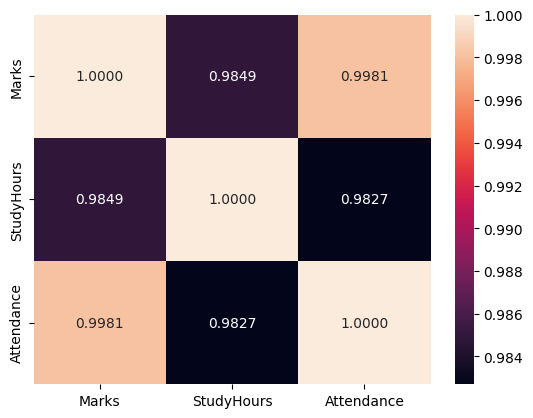
\includegraphics[width=0.75\textwidth]{img/exp8_corrHeat.png}
    % \caption{Marks of Each Student — Bar Chart}
    % \label{fig:marks_bar}
\end{figure}

\subsection{Observation}

i. All three variable pairs show a very strong positive correlation, with Pearson's r exceeding 0.98 in every case.

ii. Marks vs Attendance has the highest correlation indicating a near-perfect linear relationship.

iii. Both the Marks vs StudyHours and StudyHours vs Attendance are also very strongly correlated. This confirm that all three variable are mutually reinforcing variable.

iv. The high coefficient values suggest that the dataset is very clean and has a linear structure.